\documentclass[12pt]{article}

\usepackage{sbc-template}

\usepackage{graphicx,url}

\usepackage[utf8]{inputenc}  

\sloppy

\title{Benchmarking the Free Tier Instances of AWS}

\author{Serapheim N. Dimitropoulos}

\address{Illinois Institute of Technology
  \email{sdimitro@hawk.iit.edu}
}

\begin{document} 

\maketitle

\begin{abstract}
I benchmarked a t2.micro instance from Amazon Web Services (AWS)
and I present my results on this paper. My main objective was to
measure a series of selected metrics of the CPU, memory and disk.
In order to do that, I used programs that I wrote and
specifically tailored to get the most out of the instance,
and pre-existing performance tools and software. The main goal
of this attempt was to see how close are my measuments to the
theoritical peak performance and set a baseline for the expecation
of people interested on using Amazon's free tier instances.
Like almost all benchmarks, there aren't any conclusions to
be drawn and my results are just presented to bias the user's
expectations of the system.

\end{abstract}

\section{Motivation}
Besides the fact that most parts of this report were needed for
a programming assignment of a Cloud Computing course that I'm
currently taking, benchmarking AWS instances is an interesting
problem in its own right. Bryan Cantrill, CTO of Joyent (a company
specializing in application virtualization and cloud computing)
said: "Virtualization is a euphemism for pathological lying".
Even though Cantrill did not have AWS specifically in mind,
the main idea stays the same.
\textbf{At AWS, instances are described by hardware characteristics
like their software runs on bare metal, while in reality it runs
on virtual, software-defined boundaries}. The reasons behind
this approach are not in the scope of this paper. The interesting
part is, how much raw performance can an AWS customer get
from these instances and does this performance compare to the
hardware characteristics described when acquiring such an
instance.

\section{The Setup}
All the benchmarks took place on the free tier of the AWS cloud.
According to Amazon $\cite{amzn:1}$, all T2 instances are Burstable
Performance Instances, which means that they generally provide
some baseline performance with the ability to occasionally
burst above that baseline when needed and in accordance to
some policy. Therefore, these instances are good for workloads
that don't use the full CPU often and consistenly but they
occasionally need to burst. For my experiments I will be
measuring the performance that I get during the actual
burst as I try to bring the CPU to its limits.

The t2.micro instance that I use boasts 1 virtual
CPU of a high frequency Intel Xeon processor with Turbo up
to 3.3 GHz, 1GiB of RAM and 30GB of magnetic storage in
Amazon's Elastic Block Storage (EBS). It runs Amazon Linux
and it has a customized version of of the 4.1.13 version
of the Linux kernel. The gcc version provided with my instance
is 4.8.3 and it was compiled by Red Hat.

Examining /proc/cpuinfo from within my instance, I see that
I am running on top of Xen with an Intel Xeon E5-2670 v2 at
2.5GHz. Looking up the processor's specification on Intel
$\cite{intel:1}$, I see that this is a 64-bit 10-core processor (20 vCPUs)
with a base frequency of 2.5GHz and Max Turbo frequency
of 3.3 GHz, just as advertized from Amazon. So from the
20 vCPUs I'm given one with 64KB of L1 data and instruction
cache, 256KB L2 cache and a 25MB Intel Smart Cache, which is
basically and L3 cache that my instance will share with
all the other instances running on the same physical
machine. Unfortunately, the latter bit of information
emphasizes the fact that the performance of my instance
depends on the timings of the bursts from the other instances
that run in the same physical machine as mine.

Running dmidecode to get more information on the memory,
I get that there is a 1 GB memory device which is expected
but no more information is specified.

Finally, poking around the system for storage information
from within the instance doesn't really provide a lot of
information on the underlying virtual or physical hardware
used. Therefore, I'll just take Amazon's word $\cite{amzn:2}$, that
there exist some hard disks somewhere behind EBS and my
instance attaches to it. Although, not very descriptive
nor detailed, this means that since EBS volumes are
network-attached disk storage, when testing *disk* I/O
I should expect the average latency and throughput to be
affected by my instance's network speed. Amazon gives a
throughput estimate of 40$\sim$90MB/s per volume and I have
one volume so that should be used as my baseline for
any comparisons.

\section{CPU Benchmarking}

\section{Memory}

\section{*Disk* Behaviour \& Analysis}

\section{General Information}

All full papers and posters (short papers) submitted to some SBC conference,
including any supporting documents, should be written in English or in
Portuguese. The format paper should be A4 with single column, 3.5 cm for upper
margin, 2.5 cm for bottom margin and 3.0 cm for lateral margins, without
headers or footers. The main font must be Times, 12 point nominal size, with 6
points of space before each paragraph. Page numbers must be suppressed.

Full papers must respect the page limits defined by the conference.
Conferences that publish just abstracts ask for \textbf{one}-page texts.

\section{First Page} \label{sec:firstpage}

The first page must display the paper title, the name and address of the
authors, the abstract in English and ``resumo'' in Portuguese (``resumos'' are
required only for papers written in Portuguese). The title must be centered
over the whole page, in 16 point boldface font and with 12 points of space
before itself. Author names must be centered in 12 point font, bold, all of
them disposed in the same line, separated by commas and with 12 points of
space after the title. Addresses must be centered in 12 point font, also with
12 points of space after the authors' names. E-mail addresses should be
written using font Courier New, 10 point nominal size, with 6 points of space
before and 6 points of space after.

The abstract and ``resumo'' (if is the case) must be in 12 point Times font,
indented 0.8cm on both sides. The word \textbf{Abstract} and \textbf{Resumo},
should be written in boldface and must precede the text.

\section{CD-ROMs and Printed Proceedings}

In some conferences, the papers are published on CD-ROM while only the
abstract is published in the printed Proceedings. In this case, authors are
invited to prepare two final versions of the paper. One, complete, to be
published on the CD and the other, containing only the first page, with
abstract and ``resumo'' (for papers in Portuguese).

\section{Sections and Paragraphs}

Section titles must be in boldface, 13pt, flush left. There should be an extra
12 pt of space before each title. Section numbering is optional. The first
paragraph of each section should not be indented, while the first lines of
subsequent paragraphs should be indented by 1.27 cm.

\subsection{Subsections}

The subsection titles must be in boldface, 12pt, flush left.

\section{Figures and Captions}\label{sec:figs}


Figure and table captions should be centered if less than one line
(Figure~\ref{fig:exampleFig1}), otherwise justified and indented by 0.8cm on
both margins, as shown in Figure~\ref{fig:exampleFig2}. The caption font must
be Helvetica, 10 point, boldface, with 6 points of space before and after each
caption.

\begin{figure}[ht]
\centering
\includegraphics[width=.5\textwidth]{test.png}
\caption{A typical figure}
\label{fig:exampleFig3}
\end{figure}

\begin{figure}[ht]
\centering
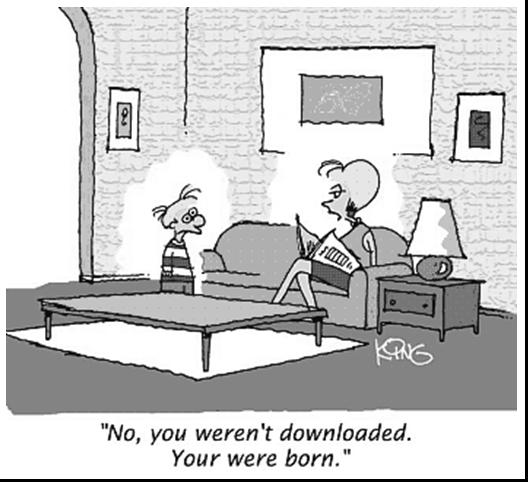
\includegraphics[width=.5\textwidth]{fig1.jpg}
\caption{A typical figure}
\label{fig:exampleFig1}
\end{figure}

\begin{figure}[ht]
\centering
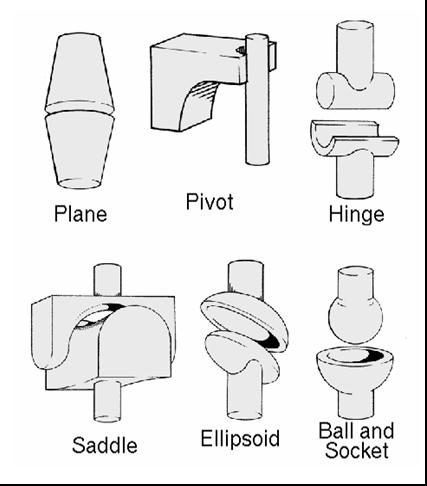
\includegraphics[width=.3\textwidth]{fig2.jpg}
\caption{This figure is an example of a figure caption taking more than one
  line and justified considering margins mentioned in Section~\ref{sec:figs}.}
\label{fig:exampleFig2}
\end{figure}

In tables, try to avoid the use of colored or shaded backgrounds, and avoid
thick, doubled, or unnecessary framing lines. When reporting empirical data,
do not use more decimal digits than warranted by their precision and
reproducibility. Table caption must be placed before the table (see Table 1)
and the font used must also be Helvetica, 10 point, boldface, with 6 points of
space before and after each caption.

\begin{table}[ht]
\centering
\caption{Variables to be considered on the evaluation of interaction
  techniques}
\label{tab:exTable1}
\smallskip
\begin{tabular}{|l|c|c|}
\hline
& Value 1 & Value 2\\[0.5ex]
\hline
&&\\[-2ex]
Case 1 & 1.0 $\pm$ 0.1 & 1.75$\times$10$^{-5}$ $\pm$ 5$\times$10$^{-7}$\\[0.5ex]
\hline
&&\\[-2ex]
Case 2 & 0.003(1) & 100.0\\[0.5ex]
\hline
\end{tabular}
\end{table}

\section{Images}

All images and illustrations should be in black-and-white, or gray tones,
excepting for the papers that will be electronically available (on CD-ROMs,
internet, etc.). The image resolution on paper should be about 600 dpi for
black-and-white images, and 150-300 dpi for grayscale images.  Do not include
images with excessive resolution, as they may take hours to print, without any
visible difference in the result. 

\section{References}

1) https://aws.amazon.com/ec2/instance-types/
2) http://ark.intel.com/products/75275/Intel-Xeon-Processor-E5-2670-v2-25M-Cache-2\_50-GHz
3) https://aws.amazon.com/ebs/details/

Bibliographic references must be unambiguous and uniform.  We recommend giving
the author names references in brackets, e.g. \cite{knuth:84},
\cite{boulic:91}, and \cite{smith:99}.

The references must be listed using 12 point font size, with 6 points of space
before each reference. The first line of each reference should not be
indented, while the subsequent should be indented by 0.5 cm.

\bibliographystyle{sbc}
\bibliography{sbc-template}

\end{document}
